\chapter{F-engine design}
\label{chap:fengine}

The development of the F-engine firmware for this project utilized the Xilinx® System Generator for DSP \citep{Xilinx_UG948_2020}. This process combined Simulink® and Xilinx blocks with components from the \gls{casper}\footnote{\url{https://casper.berkeley.edu/wiki/Main_Page}} framework, enabling an efficient and modular design approach. CASPER offers a library of pre-built modules for common DSP operations, such as FFTs, PFBs, and filtering, that can be easily combined to implement complex signal processing pipelines for radio astronomy applications \citep{hickish2016decadedevelopingradioastronomyinstrumentation,Parsons_2008}.

This methodology enables the design of digital architectures through functional blocks and visual connections, simplifying development compared to traditional hardware description languages such as VHDL or Verilog. The System Generator toolflow also includes a simulation and compilation process that translates the Simulink designs into synthesizable \gls{hdl} code, which can then be implemented on \glspl{fpga}. Nevertheless, some custom \gls{hdl} coding was necessary to implement specific functionalities not covered by existing CASPER/Xilinx blocks.

This chapter details the design of the F-engine for the \gls{charts} telescope, covering the overall architecture, the digitization and channelization chain, spectral reordering, data transmission to the X-engine and generation of local oscillators for the mixers in the FDM stage. 

\section{F-engine requirements}
\label{sec:f_engine_architecture}

As described in \S\ref{sec:charts_digital_backend}, the CHARTS digital backend employs an FX correlator architecture, where the F-engine performs initial channelization of the digitized antenna signals multiplexed by the \gls{fdm} boards. A general block diagram of the F-engine architecture is shown in Figure~\ref{fig:f_engine_block_diagram}. The design processes 32 antenna signals, each sampled at \SI{4.9152}{\giga\hertz} in quadrature mode I/Q by the RFSoC ADCs. The digitized data is first channelized using a biplex \gls{pfb} with 4 taps, producing 8192 frequency channels per stream. The outputs are then fed into a 4-stream FFT block, which computes the Fourier transform for each stream in parallel. The resulting spectra are re-quantized to a compact 4+4 bit format before being transmitted via a QSFP28 optical interface at \SI{51.2}{\giga\bit\per\second}. The design also includes custom blocks for spectral reordering which performs the corner turn and data formatting to ensure compatibility with the X-engine.

The design specifications (as stated in the objectives) for the F-engine were established as follows:

\begin{itemize}
    \item Operate over a bandwidth of at least \SI{2366}{\mega\hertz}, covering the full band delivered by the FDM stage. 
    \item Internally generate local oscillators for the FDM mixers, using the \gls{rfsoc} DAC ports. 
    \item Quantize spectral outputs into a compact 4+4 bit format, representing the real and imaginary components of each frequency channel.  
    \item Provide high-throughput data transmission using a QSFP28 optical interface, supporting \SI{100}{\giga\bit\per\second} links.  
    \item Implement spectral reordering logic to discard non-useful channels (e.g., below \SI{300}{\mega\hertz} or in the guard regions between FDM sub-bands).  
\end{itemize}

These requirements shaped the architecture, and each design decision is discussed in the following sections. 


\begin{figure}[htbp]
	\centering
	\begin{tikzpicture}
	% Paths, nodes and wires:
	\node[shape=rectangle, draw, line width=1pt, minimum width=2.298cm, minimum height=1.798cm] at (7.167, 5.5){} node[anchor=center, align=center, text width=1.91cm, inner sep=6pt] at (7.167, 5.5){\small 4-tap \\ Biplex PFB};
	\draw (3.167, 6) to[adc] (4.167, 6);
	\draw (4.167, 6) to[multiwire] (6, 6);
	\node[shape=rectangle, minimum width=0.798cm, minimum height=0.465cm] at (5, 6.5){} node[anchor=center, align=center, text width=0.41cm, inner sep=6pt] at (5, 6.5){\scriptsize 32x8};
	\node[shape=rectangle, draw, line width=1pt, minimum width=2.131cm, minimum height=3.798cm] at (11.083, 4.5){} node[anchor=center, align=center, text width=1.743cm, inner sep=6pt] at (11.083, 4.5){\small FFT\\4 streams $N=8192$};
	\draw (4.167, 5) to[multiwire] (6, 5);
	\node[shape=rectangle, minimum width=0.798cm, minimum height=0.465cm] at (5, 5.5){} node[anchor=center, align=center, text width=0.41cm, inner sep=6pt] at (5, 5.5){\scriptsize 32x8};
	\draw (4.167, 4) to[multiwire] (6, 4);
	\draw (4.167, 3) to[multiwire] (6, 3);
	\node[shape=rectangle, minimum width=0.798cm, minimum height=0.465cm] at (5, 4.5){} node[anchor=center, align=center, text width=0.41cm, inner sep=6pt] at (5, 4.5){\scriptsize 32x8};
	\node[shape=rectangle, minimum width=0.798cm, minimum height=0.465cm] at (5, 3.5){} node[anchor=center, align=center, text width=0.41cm, inner sep=6pt] at (5, 3.5){\scriptsize 32x8};
	\node[shape=rectangle, draw, line width=1pt, minimum width=2.298cm, minimum height=1.798cm] at (7.167, 3.5){} node[anchor=center, align=center, text width=1.91cm, inner sep=6pt] at (7.167, 3.5){\small4-tap \\ Biplex PFB};
	\draw (8.333, 6) to[multiwire] (10, 6);
	\draw (8.333, 5) to[multiwire] (10, 5);
	\draw (8.333, 4) to[multiwire] (10, 4);
	\draw (8.333, 3) to[multiwire] (10, 3);
	\node[shape=rectangle, minimum width=0.798cm, minimum height=0.465cm] at (9.083, 6.5){} node[anchor=center, align=center, text width=0.41cm, inner sep=6pt] at (9.083, 6.5){\scriptsize 36x8};
	\node[shape=rectangle, minimum width=0.798cm, minimum height=0.465cm] at (9.083, 5.5){} node[anchor=center, align=center, text width=0.41cm, inner sep=6pt] at (9.083, 5.5){\scriptsize 36x8};
	\node[shape=rectangle, minimum width=0.798cm, minimum height=0.465cm] at (9.083, 4.5){} node[anchor=center, align=center, text width=0.41cm, inner sep=6pt] at (9.083, 4.5){\scriptsize 36x8};
	\node[shape=rectangle, minimum width=0.798cm, minimum height=0.465cm] at (9.083, 3.5){} node[anchor=center, align=center, text width=0.41cm, inner sep=6pt] at (9.083, 3.5){\scriptsize 36x8};
	\draw (12.167, 6) to[multiwire] (13.5, 6);
	\node[shape=rectangle, draw, line width=1pt, minimum width=1.965cm, minimum height=0.798cm] at (14.5, 6){} node[anchor=center, align=center, text width=1.577cm, inner sep=6pt] at (14.5, 6){\footnotesize Re-quant.};
	\node[shape=rectangle, draw, line width=1pt, minimum width=1.965cm, minimum height=0.798cm] at (14.5, 5){} node[anchor=center, align=center, text width=1.577cm, inner sep=6pt] at (14.5, 5){\footnotesize Re-quant.};
	\node[shape=rectangle, draw, line width=1pt, minimum width=1.965cm, minimum height=0.798cm] at (14.5, 4){} node[anchor=center, align=center, text width=1.577cm, inner sep=6pt] at (14.5, 4){\footnotesize Re-quant.};
	\node[shape=rectangle, draw, line width=1pt, minimum width=1.965cm, minimum height=0.798cm] at (14.5, 3){} node[anchor=center, align=center, text width=1.577cm, inner sep=6pt] at (14.5, 3){\footnotesize Re-quant.};
	\draw (12.167, 5) to[multiwire] (13.5, 5);
	\draw (12.167, 4) to[multiwire] (13.5, 4);
	\draw (12.167, 3) to[multiwire] (13.5, 3);
	\node[shape=rectangle, minimum width=0.798cm, minimum height=0.465cm] at (12.667, 6.5){} node[anchor=north west, align=left, text width=0.41cm, inner sep=6pt] at (12.25, 6.75){\scriptsize 62x8};
	\node[shape=rectangle, minimum width=0.798cm, minimum height=0.465cm] at (12.667, 5.5){} node[anchor=north west, align=left, text width=0.41cm, inner sep=6pt] at (12.25, 5.75){\scriptsize 62x8};
	\node[shape=rectangle, minimum width=0.798cm, minimum height=0.465cm] at (12.667, 4.5){} node[anchor=north west, align=left, text width=0.41cm, inner sep=6pt] at (12.25, 4.75){\scriptsize 62x8};
	\node[shape=rectangle, minimum width=0.798cm, minimum height=0.465cm] at (12.667, 3.5){} node[anchor=north west, align=left, text width=0.41cm, inner sep=6pt] at (12.25, 3.75){\scriptsize 62x8};
	\draw (3.167, 5) to[adc] (4.167, 5);
	\draw (3.167, 4) to[adc] (4.167, 4);
	\draw (3.167, 3) to[adc] (4.167, 3);
	\node[shape=rectangle, draw, line width=1pt, dash pattern={on 4pt off 4pt}, minimum width=1.298cm, minimum height=2.131cm] at (3.667, 5.583){};
	\node[shape=rectangle, draw, line width=1pt, dash pattern={on 4pt off 4pt}, minimum width=1.298cm, minimum height=2.131cm] at (3.667, 3.417){};
	\node[shape=rectangle, minimum width=1.506cm, minimum height=0.465cm] at (3.563, 6.917){} node[anchor=west, align=left, text width=1.118cm, inner sep=6pt] at (2.792, 6.917){\scriptsize Tile 224};
	\node[shape=rectangle, minimum width=1.506cm, minimum height=0.465cm] at (3.563, 2.083){} node[anchor=west, align=left, text width=1.118cm, inner sep=6pt] at (2.792, 2.083){\scriptsize Tile 226};
	\draw (15.5, 6) to[multiwire] (16.5, 6);
	\node[shape=rectangle, minimum width=0.798cm, minimum height=0.465cm] at (16, 6.5){} node[anchor=north west, align=left, text width=0.41cm, inner sep=6pt] at (15.583, 6.75){\scriptsize 8x8};
	\node[shape=rectangle, draw, line width=1pt, minimum width=2.465cm, minimum height=3.798cm] at (17.75, 4.583){} node[anchor=center, align=center, text width=2.077cm, inner sep=6pt] at (17.75, 4.583){\small Corner-turn\\Packetizer};
	\draw (15.5, 5) to[multiwire] (16.5, 5);
	\draw (15.5, 4) to[multiwire] (16.5, 4);
	\draw (15.5, 3) to[multiwire] (16.5, 3);
	\node[shape=rectangle, minimum width=0.798cm, minimum height=0.465cm] at (16, 5.5){} node[anchor=north west, align=left, text width=0.41cm, inner sep=6pt] at (15.583, 5.75){\scriptsize 8x8};
	\node[shape=rectangle, minimum width=0.798cm, minimum height=0.465cm] at (16, 4.5){} node[anchor=north west, align=left, text width=0.41cm, inner sep=6pt] at (15.583, 4.75){\scriptsize 8x8};
	\node[shape=rectangle, minimum width=0.798cm, minimum height=0.465cm] at (16, 3.5){} node[anchor=north west, align=left, text width=0.41cm, inner sep=6pt] at (15.583, 3.75){\scriptsize 8x8};
\end{tikzpicture}
	\caption[Block diagram of the F-engine architecture]{Block diagram of the F-engine architecture. The design processes 32 antenna signals, where each ADC is sampled at \SI{4.9152}{\giga\hertz} in quadrature mode I/Q. The digitized data is first channelized using a biplex \gls{pfb} with 4 taps, producing 8192 frequency channels per stream. The outputs are then fed into a 4-stream FFT block, which computes the Fourier transform for each stream in parallel. The resulting spectra are re-quantized to a compact 4+4 bit format before being transmitted via a QSFP28 optical interface at \SI{100}{\giga\bit\per\second}. The design also includes custom blocks for spectral reordering and data formatting to ensure compatibility with the X-engine.}
	\label{fig:f_engine_block_diagram}
\end{figure}


\section{Digitization}
\label{sec:digitization}
The digitization strategy for CHARTS was carefully designed to meet the system requirements while ensuring architectural compatibility. To achieve this, the RFSoC 4x2's \gls{rfdc} was configured in quadrature (I/Q) mode. This approach was chosen because real sampling would have required a rate exceeding twice the target bandwidth ($ \SI{2366.4}{\mega\hertz}$), which, although within the ADC's maximum capability of 5 Gsps, would not allow a power-of-two number of parallel samples, something that is crucial for the posterior PFB/FFT. Quadrature sampling with decimation provided an efficient solution, as it enables the effective processed bandwidth to match the sampling frequency, fully capturing the required band while adhering to the RFDC's architectural constraints.

The sampling rate was therefore fixed at $\nu_s=\SI{4.9152}{\giga\hertz}$, comfortably covering the \SI{2366}{\mega\hertz} input band produced by the FDM stage. An internal NCO at \SI{-1.2288}{\giga\hertz} downconverts the signal to baseband, producing complex I/Q outputs centered at 0 Hz. To reduce the data rate and allow a power-of-two number of parallel samples, a decimation factor of 2 was applied, resulting in a usable baseband bandwidth of \SI{2457.6}{\mega\hertz}. This configuration is illustrated in Figure~\ref{fig:quadrature_sampling_rfdc}, which shows how the input spectrum is progressively shifted and decimated into the final baseband representation.

\begin{figure}[htbp]
    \centering
    \includegraphics[width=\textwidth]{../figures/quadrature_sampling_rfdc.pdf}
    \caption[Illustration of the frequency-domain behavior of the signal across processing stages done by the RFDC]{Illustration of the frequency-domain behavior of the signal across processing stages done by the RFDC. The top panel shows the original analog signal obtained through FDM (with each rectangle representing an antenna signal), occupying the first Nyquist zone between $0$ and $\nu_s/2$. The second panel corresponds to the digitized signal, where aliasing replicas appear both in the negative Nyquist zone ($-\nu_s/2$ to $0$) and in the second Nyquist zone ($\nu_s/2$ to $\nu_s$), as expected from sampling. The third panel illustrates the effect of mixing with a NCO at $-\nu_s/4$ (see Figure \ref{fig:quadrature_sampling}), which shifts the spectrum and redistributes its content symmetrically across the Nyquist regions. The bottom panel shows the result after decimation by a factor of two, where the spectrum is compressed into half the bandwidth, now spanning from $-\nu_s/4$ to $+\nu_s/4$.}
    \label{fig:quadrature_sampling_rfdc}
\end{figure}

Since the system must simultaneously digitize 32 antennas, with 8 signals multiplexed per ADC, all converters available in the RFSoC 4x2 are used. In particular, the dual tiles 224 and 226 were enabled and configured for quadrature sampling (see Figure \ref{fig:rfsoc_tiles} for tile organization of ADCs). Table \ref{tab:rfdc_config} summarizes the configuration parameters for each ADC.


\begin{table}[htbp]
\centering
\begin{tabular}{lc}
\toprule
Parameter & Value \\
\midrule
Sampling rate $\nu_s$ & 4915.2 Msps \\
Reference clock & 307.2 MHz \\
Digital Output & I/Q \\
Decimation Mode & 2x \\
Samples per Cycle & 8 \\
Mixer Type & Fine \\
Mixer Mode & Real $\rightarrow$ I/Q \\
NCO Frequency & $-1.2288$ GHz \\
NCO Phase & 0 \\
Nyquist Zone & Zone 1 \\
Calibration Mode & Mode 2 \\
\bottomrule
\end{tabular}
\caption{Configuration parameters of the RFSoC 4x2 RFDC ADC dual tiles (224 and 226).}
\label{tab:rfdc_config}
\end{table}


With these configurations, the output data rate is \SI{256}{bits} per clock cycle, corresponding to 8 complex I/Q samples of \SI{32}{bits} each (16 + 16 signed), giving a required AXI4-Stream clock frequency of \SI{307.2}{\mega\hertz} to sustain the \SI{2457.6}{\mega\hertz} bandwidth. In order to produce this sample clock in the ADC tiles of the RFSoC, the Texas Instruments LMX2594 RF synthesizer was configured to generate a \SI{307.2}{\mega\hertz} reference, used by the ADC tile. This frequency is different from the \SI{491.52}{\mega\hertz} default reference clock provided in every CASPER image instance (\texttt{rfsoc4x2rfsoc4x2\_LMX\_REF\_245M76\_OUT\_491M52.txt} file), but due to harmonics of this clock appearing after channelization, it was changed to \SI{307.2}{\mega\hertz} so that the spurious tone falls exactly on an FFT bin, simplifying its removal in later stages.

Since for dual-tile platforms in I/Q digital output modes the in-phase and quadrature data are produced from different ports, before channelization the data stream is reordered using the CASPER \texttt{munge} block into the format $[I_1, Q_1, I_2, Q_2, \dots]$, ensuring compatibility with downstream processing blocks.


\section{LO generation}

The \glspl{lo} are a key element in the \gls{fdm} architecture, as they enable the upconversion of the 300--500 MHz signals from the antennas into higher frequency bands ranging from 300 to $\sim 2366$ MHz. Since the RFSoC 4x2 incorporates high-speed \glspl{dac}, these were used to synthesize the \glspl{lo} digitally and output them directly in the analog domain. This choice avoids the need for external frequency synthesizers, while providing high flexibility and real-time configurability.

The system requires four independent \glspl{lo} at 1065.6, 1332, 1600.8 and 1864.8 MHz, in phase. The rationale behind these values will be discussed later in the channelization section (\S\ref{sec:channelization}), but they were chosen to satisfy the bandwidth and frequency placement requirements of the instrument.

The \gls{dac} tiles were configured similarly to the \gls{adc} tiles, but operating in real-to-real mode without interpolation. Each tile outputs 16 parallel 16-bit samples per clock cycle, with a sampling rate of \SI{4915.2}{\mega\hertz}, therefore the AXI4-Stream clock frequency is also set to \SI{307.2}{\mega\hertz} to match the ADC sample clock. The DAC output is thus a real-valued waveform with a Nyquist frequency of \SI{2457.6}{\mega\hertz}, which is sufficient to cover the highest required \gls{lo} frequency of \SI{1864.8}{\mega\hertz}. The configuration parameters of the DAC tiles are summarized in Table~\ref{tab:dac_config}.
\begin{table}[htbp]
\centering
\begin{tabular}{lc}
\toprule
Parameter & Value \\
\midrule
Sampling rate $\nu_s$ & 4915.2 Msps \\
Reference clock & 307.2 MHz \\
Digital Input & Real \\
Interpolation Mode & None \\
Samples per Cycle & 16 \\
Nyquist Zone & Zone 1 \\
Calibration Mode & Mode 2 \\
\bottomrule
\end{tabular}
\caption{Configuration parameters of the RFSoC 4x2 RFDC DAC tiles (228 and 230).}
\label{tab:dac_config}
\end{table}


The generation of the \glspl{lo} is based on the digital synthesis of four sinusoidal tones per \gls{dac}. Each tone has programmable frequency and amplitude, and all are summed digitally to form a composite signal. At the analog stage, external band-pass filters are used to isolate the desired frequency component, ensuring that each mixer receives its corresponding \gls{lo}.

The tones are synthesized using lookup tables stored in block RAM, which contain the sampled values of a sine function. These are addressed by phase accumulators operating at the system clock, where the phase increment determines the output frequency. Amplitude control is achieved by applying digital attenuations to the waveform samples before summation. Both frequency and attenuation parameters are mapped to software-controlled registers, enabling their adjustment in real time. Credits to Frederik Brecht from University of Toronto for the original tone generator design, later optimized and adapted by the author.

Figure~\ref{fig:lo_generation} illustrates the architecture of the \gls{lo} generation block. Both DAC tiles contain a sum of four tones. The outputs are connected to the appropriate pins on the RFSoC board (DAC A and DAC B), which are routed to SMA connectors for external filtering and distribution to the FDM boards.

\begin{figure}[h!]
\centering


\tikzset{every picture/.style={line width=0.75pt}} %set default line width to 0.75pt        

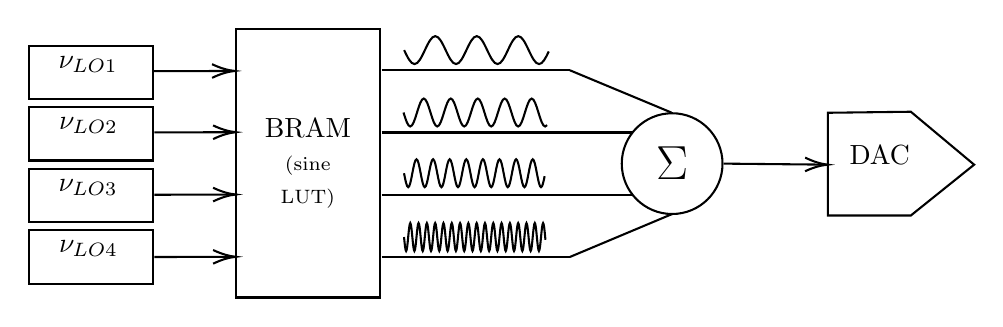
\begin{tikzpicture}[x=0.75pt,y=0.75pt,yscale=-1,xscale=1]
%uncomment if require: \path (0,216); %set diagram left start at 0, and has height of 216

%Shape: Wave [id:dp8030811849314586] 
\draw   (220.88,70.3) .. controls (222.51,73.75) and (224.07,77.03) .. (225.88,77.03) .. controls (227.69,77.03) and (229.25,73.75) .. (230.88,70.3) .. controls (232.51,66.86) and (234.07,63.58) .. (235.88,63.58) .. controls (237.69,63.58) and (239.25,66.86) .. (240.88,70.3) .. controls (242.51,73.75) and (244.07,77.03) .. (245.88,77.03) .. controls (247.69,77.03) and (249.25,73.75) .. (250.88,70.3) .. controls (252.51,66.86) and (254.07,63.58) .. (255.88,63.58) .. controls (257.69,63.58) and (259.25,66.86) .. (260.88,70.3) .. controls (262.51,73.75) and (264.07,77.03) .. (265.88,77.03) .. controls (267.69,77.03) and (269.25,73.75) .. (270.88,70.3) .. controls (272.51,66.86) and (274.07,63.58) .. (275.88,63.58) .. controls (277.69,63.58) and (279.25,66.86) .. (280.88,70.3) .. controls (282.51,73.75) and (284.07,77.03) .. (285.88,77.03) .. controls (287.57,77.03) and (289.04,74.17) .. (290.56,70.98) ;
%Shape: Rectangle [id:dp14290550899959387] 
\draw   (140,60) -- (209.47,60) -- (209.47,189.5) -- (140,189.5) -- cycle ;
%Shape: Rectangle [id:dp4738866346988476] 
\draw   (40,68.23) -- (99.93,68.23) -- (99.93,94) -- (40,94) -- cycle ;

%Straight Lines [id:da08918771819995541] 
\draw    (100,80.47) -- (137.28,80.36) ;
\draw [shift={(139.28,80.35)}, rotate = 179.83] [color={rgb, 255:red, 0; green, 0; blue, 0 }  ][line width=0.75]    (10.93,-3.29) .. controls (6.95,-1.4) and (3.31,-0.3) .. (0,0) .. controls (3.31,0.3) and (6.95,1.4) .. (10.93,3.29)   ;
%Shape: Rectangle [id:dp8436306464725387] 
\draw   (40.17,97.73) -- (100.1,97.73) -- (100.1,123.5) -- (40.17,123.5) -- cycle ;

%Straight Lines [id:da20670514517993] 
\draw    (100.5,109.97) -- (137.78,109.86) ;
\draw [shift={(139.78,109.85)}, rotate = 179.83] [color={rgb, 255:red, 0; green, 0; blue, 0 }  ][line width=0.75]    (10.93,-3.29) .. controls (6.95,-1.4) and (3.31,-0.3) .. (0,0) .. controls (3.31,0.3) and (6.95,1.4) .. (10.93,3.29)   ;
%Shape: Rectangle [id:dp24967622455401983] 
\draw   (40,127.57) -- (99.93,127.57) -- (99.93,153.33) -- (40,153.33) -- cycle ;

%Straight Lines [id:da8954020601514457] 
\draw    (100.5,140) -- (137.78,139.89) ;
\draw [shift={(139.78,139.88)}, rotate = 179.83] [color={rgb, 255:red, 0; green, 0; blue, 0 }  ][line width=0.75]    (10.93,-3.29) .. controls (6.95,-1.4) and (3.31,-0.3) .. (0,0) .. controls (3.31,0.3) and (6.95,1.4) .. (10.93,3.29)   ;
%Shape: Rectangle [id:dp9537613021306607] 
\draw   (40.17,157.07) -- (100.1,157.07) -- (100.1,182.83) -- (40.17,182.83) -- cycle ;

%Straight Lines [id:da8044392081502272] 
\draw    (100.5,170) -- (137.78,169.89) ;
\draw [shift={(139.78,169.88)}, rotate = 179.83] [color={rgb, 255:red, 0; green, 0; blue, 0 }  ][line width=0.75]    (10.93,-3.29) .. controls (6.95,-1.4) and (3.31,-0.3) .. (0,0) .. controls (3.31,0.3) and (6.95,1.4) .. (10.93,3.29)   ;
%Shape: Wave [id:dp333884189071195] 
\draw   (220.58,100.37) .. controls (221.64,103.82) and (222.66,107.1) .. (223.83,107.1) .. controls (225.01,107.1) and (226.02,103.82) .. (227.08,100.37) .. controls (228.14,96.93) and (229.16,93.65) .. (230.33,93.65) .. controls (231.51,93.65) and (232.52,96.93) .. (233.58,100.37) .. controls (234.64,103.82) and (235.66,107.1) .. (236.83,107.1) .. controls (238.01,107.1) and (239.02,103.82) .. (240.08,100.37) .. controls (241.14,96.93) and (242.16,93.65) .. (243.33,93.65) .. controls (244.51,93.65) and (245.52,96.93) .. (246.58,100.37) .. controls (247.64,103.82) and (248.66,107.1) .. (249.83,107.1) .. controls (251.01,107.1) and (252.02,103.82) .. (253.08,100.37) .. controls (254.14,96.93) and (255.16,93.65) .. (256.33,93.65) .. controls (257.51,93.65) and (258.52,96.93) .. (259.58,100.37) .. controls (260.64,103.82) and (261.66,107.1) .. (262.83,107.1) .. controls (264.01,107.1) and (265.02,103.82) .. (266.08,100.37) .. controls (267.14,96.93) and (268.16,93.65) .. (269.33,93.65) .. controls (270.51,93.65) and (271.52,96.93) .. (272.58,100.37) .. controls (273.64,103.82) and (274.66,107.1) .. (275.83,107.1) .. controls (277.01,107.1) and (278.02,103.82) .. (279.08,100.37) .. controls (280.14,96.93) and (281.16,93.65) .. (282.33,93.65) .. controls (283.51,93.65) and (284.52,96.93) .. (285.58,100.37) .. controls (286.64,103.82) and (287.66,107.1) .. (288.83,107.1) .. controls (289.15,107.1) and (289.46,106.86) .. (289.76,106.44) ;
%Shape: Wave [id:dp7393150876481582] 
\draw   (220.83,129.62) .. controls (221.49,133.07) and (222.11,136.35) .. (222.83,136.35) .. controls (223.56,136.35) and (224.18,133.07) .. (224.83,129.62) .. controls (225.49,126.18) and (226.11,122.9) .. (226.83,122.9) .. controls (227.56,122.9) and (228.18,126.18) .. (228.83,129.62) .. controls (229.49,133.07) and (230.11,136.35) .. (230.83,136.35) .. controls (231.56,136.35) and (232.18,133.07) .. (232.83,129.62) .. controls (233.49,126.18) and (234.11,122.9) .. (234.83,122.9) .. controls (235.56,122.9) and (236.18,126.18) .. (236.83,129.62) .. controls (237.49,133.07) and (238.11,136.35) .. (238.83,136.35) .. controls (239.56,136.35) and (240.18,133.07) .. (240.83,129.62) .. controls (241.49,126.18) and (242.11,122.9) .. (242.83,122.9) .. controls (243.56,122.9) and (244.18,126.18) .. (244.83,129.62) .. controls (245.49,133.07) and (246.11,136.35) .. (246.83,136.35) .. controls (247.56,136.35) and (248.18,133.07) .. (248.83,129.62) .. controls (249.49,126.18) and (250.11,122.9) .. (250.83,122.9) .. controls (251.56,122.9) and (252.18,126.18) .. (252.83,129.62) .. controls (253.49,133.07) and (254.11,136.35) .. (254.83,136.35) .. controls (255.56,136.35) and (256.18,133.07) .. (256.83,129.62) .. controls (257.49,126.18) and (258.11,122.9) .. (258.83,122.9) .. controls (259.56,122.9) and (260.18,126.18) .. (260.83,129.62) .. controls (261.49,133.07) and (262.11,136.35) .. (262.83,136.35) .. controls (263.56,136.35) and (264.18,133.07) .. (264.83,129.62) .. controls (265.49,126.18) and (266.11,122.9) .. (266.83,122.9) .. controls (267.56,122.9) and (268.18,126.18) .. (268.83,129.62) .. controls (269.49,133.07) and (270.11,136.35) .. (270.83,136.35) .. controls (271.56,136.35) and (272.18,133.07) .. (272.83,129.62) .. controls (273.49,126.18) and (274.11,122.9) .. (274.83,122.9) .. controls (275.56,122.9) and (276.18,126.18) .. (276.83,129.62) .. controls (277.49,133.07) and (278.11,136.35) .. (278.83,136.35) .. controls (279.56,136.35) and (280.18,133.07) .. (280.83,129.62) .. controls (281.49,126.18) and (282.11,122.9) .. (282.83,122.9) .. controls (283.56,122.9) and (284.18,126.18) .. (284.83,129.62) .. controls (285.49,133.07) and (286.11,136.35) .. (286.83,136.35) .. controls (287.46,136.35) and (288,133.93) .. (288.56,131.06) ;
%Shape: Wave [id:dp2438632428884676] 
\draw   (220.83,160.37) .. controls (221.16,163.82) and (221.47,167.1) .. (221.83,167.1) .. controls (222.2,167.1) and (222.51,163.82) .. (222.83,160.37) .. controls (223.16,156.93) and (223.47,153.65) .. (223.83,153.65) .. controls (224.2,153.65) and (224.51,156.93) .. (224.83,160.37) .. controls (225.16,163.82) and (225.47,167.1) .. (225.83,167.1) .. controls (226.2,167.1) and (226.51,163.82) .. (226.83,160.37) .. controls (227.16,156.93) and (227.47,153.65) .. (227.83,153.65) .. controls (228.2,153.65) and (228.51,156.93) .. (228.83,160.37) .. controls (229.16,163.82) and (229.47,167.1) .. (229.83,167.1) .. controls (230.2,167.1) and (230.51,163.82) .. (230.83,160.37) .. controls (231.16,156.93) and (231.47,153.65) .. (231.83,153.65) .. controls (232.2,153.65) and (232.51,156.93) .. (232.83,160.37) .. controls (233.16,163.82) and (233.47,167.1) .. (233.83,167.1) .. controls (234.2,167.1) and (234.51,163.82) .. (234.83,160.37) .. controls (235.16,156.93) and (235.47,153.65) .. (235.83,153.65) .. controls (236.2,153.65) and (236.51,156.93) .. (236.83,160.37) .. controls (237.16,163.82) and (237.47,167.1) .. (237.83,167.1) .. controls (238.2,167.1) and (238.51,163.82) .. (238.83,160.37) .. controls (239.16,156.93) and (239.47,153.65) .. (239.83,153.65) .. controls (240.2,153.65) and (240.51,156.93) .. (240.83,160.37) .. controls (241.16,163.82) and (241.47,167.1) .. (241.83,167.1) .. controls (242.2,167.1) and (242.51,163.82) .. (242.83,160.37) .. controls (243.16,156.93) and (243.47,153.65) .. (243.83,153.65) .. controls (244.2,153.65) and (244.51,156.93) .. (244.83,160.37) .. controls (245.16,163.82) and (245.47,167.1) .. (245.83,167.1) .. controls (246.2,167.1) and (246.51,163.82) .. (246.83,160.37) .. controls (247.16,156.93) and (247.47,153.65) .. (247.83,153.65) .. controls (248.2,153.65) and (248.51,156.93) .. (248.83,160.37) .. controls (249.16,163.82) and (249.47,167.1) .. (249.83,167.1) .. controls (250.2,167.1) and (250.51,163.82) .. (250.83,160.37) .. controls (251.16,156.93) and (251.47,153.65) .. (251.83,153.65) .. controls (252.2,153.65) and (252.51,156.93) .. (252.83,160.37) .. controls (253.16,163.82) and (253.47,167.1) .. (253.83,167.1) .. controls (254.2,167.1) and (254.51,163.82) .. (254.83,160.37) .. controls (255.16,156.93) and (255.47,153.65) .. (255.83,153.65) .. controls (256.2,153.65) and (256.51,156.93) .. (256.83,160.37) .. controls (257.16,163.82) and (257.47,167.1) .. (257.83,167.1) .. controls (258.2,167.1) and (258.51,163.82) .. (258.83,160.37) .. controls (259.16,156.93) and (259.47,153.65) .. (259.83,153.65) .. controls (260.2,153.65) and (260.51,156.93) .. (260.83,160.37) .. controls (261.16,163.82) and (261.47,167.1) .. (261.83,167.1) .. controls (262.2,167.1) and (262.51,163.82) .. (262.83,160.37) .. controls (263.16,156.93) and (263.47,153.65) .. (263.83,153.65) .. controls (264.2,153.65) and (264.51,156.93) .. (264.83,160.37) .. controls (265.16,163.82) and (265.47,167.1) .. (265.83,167.1) .. controls (266.2,167.1) and (266.51,163.82) .. (266.83,160.37) .. controls (267.16,156.93) and (267.47,153.65) .. (267.83,153.65) .. controls (268.2,153.65) and (268.51,156.93) .. (268.83,160.37) .. controls (269.16,163.82) and (269.47,167.1) .. (269.83,167.1) .. controls (270.2,167.1) and (270.51,163.82) .. (270.83,160.37) .. controls (271.16,156.93) and (271.47,153.65) .. (271.83,153.65) .. controls (272.2,153.65) and (272.51,156.93) .. (272.83,160.37) .. controls (273.16,163.82) and (273.47,167.1) .. (273.83,167.1) .. controls (274.2,167.1) and (274.51,163.82) .. (274.83,160.37) .. controls (275.16,156.93) and (275.47,153.65) .. (275.83,153.65) .. controls (276.2,153.65) and (276.51,156.93) .. (276.83,160.37) .. controls (277.16,163.82) and (277.47,167.1) .. (277.83,167.1) .. controls (278.2,167.1) and (278.51,163.82) .. (278.83,160.37) .. controls (279.16,156.93) and (279.47,153.65) .. (279.83,153.65) .. controls (280.2,153.65) and (280.51,156.93) .. (280.83,160.37) .. controls (281.16,163.82) and (281.47,167.1) .. (281.83,167.1) .. controls (282.2,167.1) and (282.51,163.82) .. (282.83,160.37) .. controls (283.16,156.93) and (283.47,153.65) .. (283.83,153.65) .. controls (284.2,153.65) and (284.51,156.93) .. (284.83,160.37) .. controls (285.16,163.82) and (285.47,167.1) .. (285.83,167.1) .. controls (286.2,167.1) and (286.51,163.82) .. (286.83,160.37) .. controls (287.16,156.93) and (287.47,153.65) .. (287.83,153.65) .. controls (288.2,153.65) and (288.51,156.93) .. (288.83,160.37) .. controls (288.88,160.82) and (288.92,161.27) .. (288.96,161.7) ;
%Straight Lines [id:da42425354625752143] 
\draw    (210,80) -- (300.67,80) ;
%Straight Lines [id:da624489699175146] 
\draw    (210,110) -- (300.67,110) ;
%Straight Lines [id:da6320159558919146] 
\draw    (210,140) -- (300.67,140) ;
%Straight Lines [id:da6042226130180868] 
\draw    (210,170) -- (300.67,170) ;
%Straight Lines [id:da1125229696814749] 
\draw    (300.67,80) -- (349.72,100.42) ;
%Straight Lines [id:da45114341559107585] 
\draw    (300,110) -- (331.26,110) ;
%Straight Lines [id:da4480014325851498] 
\draw    (300.67,170) -- (349.88,149.34) ;
%Straight Lines [id:da4754341796323369] 
\draw    (300,140) -- (330.95,140) ;
%Straight Lines [id:da2100119332647683] 
\draw    (375,125) -- (423,125.48) ;
\draw [shift={(425,125.5)}, rotate = 180.57] [color={rgb, 255:red, 0; green, 0; blue, 0 }  ][line width=0.75]    (10.93,-3.29) .. controls (6.95,-1.4) and (3.31,-0.3) .. (0,0) .. controls (3.31,0.3) and (6.95,1.4) .. (10.93,3.29)   ;
%Shape: Polygon [id:ds301056972073124] 
\draw   (465,100) -- (495.5,125.5) -- (465,150) -- (425,150) -- (425,100.5) -- cycle ;

% Text Node
\draw (52.97,71.86) node [anchor=north west][inner sep=0.75pt]   [align=left] {$\displaystyle \nu _{\text{LO1}}$};
% Text Node
\draw (53.13,101.36) node [anchor=north west][inner sep=0.75pt]   [align=left] {$\displaystyle \nu _{\text{LO2}}$};
% Text Node
\draw (53.13,160.7) node [anchor=north west][inner sep=0.75pt]   [align=left] {$\displaystyle \nu _{\text{LO4}}$};
% Text Node
\draw (52.97,131.2) node [anchor=north west][inner sep=0.75pt]   [align=left] {$\displaystyle \nu _{\text{LO3}}$};
% Text Node
\draw (174.48,124.94) node   [align=left] {\begin{minipage}[lt]{37.53pt}\setlength\topsep{0pt}
\begin{center}
{ BRAM}\\{{\scriptsize (sine LUT)}}
\end{center}

\end{minipage}};
% Text Node
\draw (450,121) node   [align=left] {\begin{minipage}[lt]{24.26pt}\setlength\topsep{0pt}
\begin{center}
DAC
\end{center}

\end{minipage}};
% Text Node
\draw    (350, 125) circle [x radius= 24.27, y radius= 24.27]   ;
\draw (350,125) node  [font=\LARGE] [align=left] {\begin{minipage}[lt]{16.41pt}\setlength\topsep{0pt}
\begin{center}
$\displaystyle \Sigma $
\end{center}

\end{minipage}};


\end{tikzpicture}

\caption[Architecture of the LO generation block]{Architecture of the \gls{lo} generation block. Four configurable registers set the frequencies of the \glspl{lo} ($\nu_{\text{LO1}}$, $\nu_{\text{LO2}}$, $\nu_{\text{LO3}}$, $\nu_{\text{LO4}}$). Each register feeds a \gls{bram} containing a sine \gls{lut}, which outputs the corresponding waveform. The outputs of the four \glspl{bram} are summed and sent to \gls{dac} tiles 228 and 230. Each \gls{dac} tile produces one independent output, each containing a sum of four tones. The outputs are connected to the appropriate pins on the RFSoC board, which are routed to SMA connectors for external filtering and distribution to the FDM boards.}
\label{fig:lo_generation}
\end{figure}


\label{sec:lo_generation}




\section{Channelization}
\label{sec:channelization}

Channelization is performed by a 4-tap PFB with convergent rounding and 18-bit coefficients. The output format of the PFB is set to 18 + 18 bits (real and imaginary parts), following CASPER design recommendations to balance precision and resource usage. 


The filtered samples are then passed to an 8192-point radix-2 pipeline FFT, which operates directly on the complex input.  The FFT is configured with automatic bit growth: at each stage of the 13-stage radix-2 pipeline, the word length increases by 1 bit to accommodate intermediate dynamic range expansion. Consequently, the final output has a format of $31 + 31$ bits, which is subsequently re-quantized according to the strategy described in \S\ref{sec:re-quantization}. As there are 13 stages the total number of channels is $2^{13} = 8192$, resulting in a channel width of \SI{300}{\kilo\hertz} over the \SI{2457.6}{\mega\hertz} bandwidth. The FFT is clocked at \SI{307.2}{\mega\hertz} with 8 samples per clock cycle, producing a new spectrum every \SI{3.33}{\micro\second}, and unlike real-input FFT architectures, no channels are discarded. 
Key specifications of the F-engine design are summarized in Table~\ref{tab:f_engine_metrics}.

\begin{table}[htbp]
\centering
\begin{tabular}{l l}
\hline
Metric & Value \\
\hline
Frequency channels & 8192 \\
Effective bandwidth & \SI{2.4576}{\giga\hertz} \\
Channel width & \SI{300}{\kilo\hertz} \\
Frame time resolution & \SI{3.33}{\micro\second}  \\
\hline
\end{tabular}
\caption[F-engine specifications]{Key specifications of the F-engine design, including the number of frequency channels, effective bandwidth, channel width, and frame time resolution.}
\label{tab:f_engine_metrics}
\end{table}

The \SI{300}{\kilo\hertz} channel width provides the spectral resolution required for the intended scientific applications and mitigates dispersion-induced broadening (DM smearing), which is more acute in lower frequencies where the dispersion is greater. In addition, the \SI{3.33}{\micro\second} frame time resolution enables high-cadence, low-latency processing, facilitating calibration and correlation of antenna signals for each of the eight FDM chains. The full band and corresponding FFT bins for each chain are listed in Table~\ref{tab:fdm_chains}, resulting in 672 channels per chain. The frequency placement of the chains was chosen so that the bands align with multiples of eight, ensuring compatibility with the FFT output, which delivers the spectrum in groups of eight samples. Note that chains 1, 2, and 3 require frequency flipping due to the mixing scheme used in the FDM stage.

\begin{table}[htbp]
\centering
\begin{tabular}{cccc}
\toprule
Chain & Frequency Range (MHz) & Bin Range & Flipped \\
\midrule
0 & 300--501.6 & 1000--1672 & No \\
1 & 564--765.6 & 1880--2552 & Yes \\
2 & 830.4--1032 & 2768--3440 & Yes \\
3 & 1099.2--1300.8 & 3664--4336 & Yes \\
4 & 1365.6--1567.2 & 4552--5224 & No \\
5 & 1632--1833.6 & 5440--6112 & No \\
6 & 1900.8--2102.4 & 6336--7008 & No \\
7 & 2164.8--2366.4 & 7216--7888 & No \\
\bottomrule
\end{tabular}
\caption[FDM chains and corresponding FFT bins]{FDM chains and corresponding FFT bins. Each of the 8 FDM chains covers a \SI{201.6}{\mega\hertz} band, with a $\sim\SI{66}{\mega\hertz}$ guard region between adjacent chains. The table lists the frequency range, FFT bin range, and the LO frequency associated with each chain.}
\label{tab:fdm_chains}
\end{table}

\section{Re-quantization and calibration}
\label{sec:re-quantization}

The FFT output produces complex samples with a precision of 31+31 bits per channel, which must be reduced before transmission to the X-engine. To achieve this, the system applies a re-quantization step that truncates the data stream to 4+4 bits. Although this quantization inevitably leads to some information loss, in practice the effect is small for typical radio astronomy signals and is compensated by the advantages of reducing the data volume. The lower bit depth enables higher bandwidth coverage and efficient real-time processing, while keeping quantization-induced biases within negligible levels.

Quantization, however, introduces systematic effects in both amplitude and phase of the measured correlations, which in turn impact calibration accuracy and the fidelity of reconstructed images. To minimize these effects, the system applies a digital gain and scaling stage prior to truncation. The calibration aims to adjust each frequency channel such that the signal level is close to 1 bit RMS (approximately two quantization steps). In this regime, the correlation between the signal and the quantization error becomes vanishingly small, the increase in output variance is only about 4\%, and the resulting bias in correlation measurements falls below $10^{-6}$ in magnitude and $10^{-11}$ degrees in phase (see \citealt{menaparra2018quantizationbiasdigitalcorrelators} for a detailed analysis of quantization effects in radio interferometry).

The calibration process operates in three steps, as illustrated in Figure~\ref{fig:quantizer_architecture}. First, the 31+31 bit FFT output of each channel is multiplied by a 16-bit programmable gain factor, applied identically to the real and imaginary components. This stage allows fine adjustment of the signal amplitude per channel. The result is a 48+48\footnote{The additional bit for real and imaginary parts comes from the signed extension of the gain value to 17 bits.} bit word, which is then shifted left by a configurable number of bits (equivalent to multiplying by powers of two). This left shift is applied uniformly across all frequency channels and serves to optimize the dynamic range before truncation. Finally, the system selects the 4 most significant bits of the real and imaginary components and applies convergent rounding-to-even following the UG901 guidelines \citep{Xilinx_UG901_2025} for hardware efficiency coding, yielding a compact 4+4 bit representation per channel. A clipping flag is raised whenever a value with integer part equal to 0111 (decimal 7) and a non-zero fractional component reaches the rounding stage\footnote{The possible range of values for a 4 bit signed number is $[-8,7]$, hence the need for clipping.}, providing diagnostics for potential saturation.

\begin{figure}[htbp]
    \centering
    \begin{tikzpicture}
	% Paths, nodes and wires:
	\node[shape=rectangle, minimum width=1.131cm, minimum height=0.631cm] at (5.983, 2.4){} node[anchor=center, align=center, text width=0.743cm, inner sep=6pt] at (5.983, 2.4){$g$};
	\node[mixer] at (6, 4){};
	\node[shape=rectangle, draw, line width=1pt, minimum width=1.215cm, minimum height=0.965cm] at (8.375, 4){} node[anchor=center, align=center, text width=0.827cm, inner sep=6pt] at (8.375, 4){$<<$};
	\draw[-latex] (6, 2.667) -- (6, 3.51);
	\node[shape=rectangle, minimum width=1.131cm, minimum height=0.631cm] at (4.75, 4.917){} node[anchor=center, align=center, text width=0.743cm, inner sep=6pt] at (4.75, 4.917){\small 31+31};
	\node[shape=rectangle, minimum width=0.765cm, minimum height=0.298cm] at (6.35, 3){} node[anchor=center, align=center, text width=0.377cm, inner sep=6pt] at (6.35, 3){\small 16};
	\node[shape=rectangle, minimum width=1.131cm, minimum height=0.631cm] at (7.25, 4.917){} node[anchor=center, align=center, text width=0.743cm, inner sep=6pt] at (7.25, 4.917){\small 48+48};
	\node[shape=rectangle, minimum width=0.565cm, minimum height=0.365cm] at (4.8, 3.8){} node[anchor=center, align=center, text width=0.177cm, inner sep=6pt] at (4.8, 3.8){\scriptsize 8};
	\node[shape=rectangle, minimum width=0.565cm, minimum height=0.365cm] at (7.2, 3.8){} node[anchor=center, align=center, text width=0.177cm, inner sep=6pt] at (7.2, 3.8){\scriptsize 8};
	\node[shape=rectangle, minimum width=1.131cm, minimum height=0.631cm] at (8.333, 2.167){} node[anchor=center, align=center, text width=0.743cm, inner sep=6pt] at (8.333, 2.167){dynamic\\shifter};
	\draw[-latex] (8.375, 2.657) -- (8.375, 3.5);
	\node[shape=rectangle, minimum width=0.565cm, minimum height=0.365cm] at (9.8, 3.8){} node[anchor=center, align=center, text width=0.177cm, inner sep=6pt] at (9.8, 3.8){\scriptsize 8};
	\node[shape=rectangle, draw, line width=1pt, minimum width=1.455cm, minimum height=0.765cm] at (11.255, 4){} node[anchor=center, align=center, text width=1.067cm, inner sep=6pt] at (11.255, 4){round};
	\node[shape=rectangle, minimum width=1.131cm, minimum height=0.631cm] at (9.75, 4.917){} node[anchor=center, align=center, text width=0.743cm, inner sep=6pt] at (9.75, 4.917){\small 48+48};
	\draw (4, 4) to[multiwire] (5.51, 4);
	\draw (6.49, 4) to[multiwire] (7.75, 4);
	\draw (9, 4) to[multiwire] (10.51, 4);
	\draw (12, 4) to[multiwire] (13.5, 4);
	\node[ocirc] at (13.5, 4){};
	\node[shape=rectangle, minimum width=0.565cm, minimum height=0.365cm] at (12.8, 3.8){} node[anchor=center, align=center, text width=0.177cm, inner sep=6pt] at (12.8, 3.8){\scriptsize 8};
	\node[shape=rectangle, minimum width=1.131cm, minimum height=0.631cm] at (12.667, 4.917){} node[anchor=center, align=center, text width=0.743cm, inner sep=6pt] at (12.667, 4.917){\small 4+4};
	\node[shape=rectangle, minimum width=0.765cm, minimum height=0.298cm] at (8.75, 3){} node[anchor=center, align=center, text width=0.377cm, inner sep=6pt] at (8.75, 3){\small 5};
	\node[shape=rectangle, draw, line width=1pt, minimum width=1.215cm, minimum height=0.965cm] at (3.375, 4){} node[anchor=center, align=center, text width=0.827cm, inner sep=6pt] at (3.375, 4){FFT};
\end{tikzpicture}
    \caption[Schematic of the quantization process]{Schematic of the quantization process. The 31+31 bit FFT output is first multiplied by a 16-bit programmable gain factor $g$, resulting in a 48+48 bit word. This is then shifted left by a configurable number of bits (up to 5 bits) to optimize dynamic range. Finally, the most significant 4 bits of the real and imaginary components are selected, with convergent rounding-to-even applied to yield a compact 4+4 bit representation per channel. A clipping flag is raised if saturation occurs during rounding.}
    \label{fig:quantizer_architecture}
\end{figure}



The combination of the programmable per-channel gain and the global left shift defines the effective digital gain applied in the calibration stage. These parameters are software-configurable, allowing flexible tuning of the re-quantization pipeline. The calibration gains are initially computed by measuring the RMS power of the channelized data for each input and frequency channel, ensuring that the levels are brought close to the desired 1 bit RMS target. Subsequently, the per-channel gains are smoothed across frequency using an iterative algorithm that combines polynomial fitting with Fourier-based filtering. This smoothing suppresses unphysical channel-to-channel variations while preserving real spectral structure.

In practice, the digital gain calibration needs to be performed only once for each input and frequency channel under stable observing conditions. Updates may be required if instrumental responses drift significantly over time or if the RFI environment changes.

\section{Spectral reordering}
\label{sec:spectral_reordering}


\section{Packetization and data transmission}

\label{sec:packetization}

\begin{table}[htbp]
\centering
\label{tab:packet_format}
\begin{tabular}{lll}
\toprule
\textbf{Field} & \textbf{Size (bytes)} & \textbf{Description} \\
\midrule
MCNT           & 8   & Monotonic counter, increments by 1 for each packet sent. \\
ADC ID         & 1   & Identifier of ADC source (0--3). \\
Num channels   & 2   & Number of frequency channels carried (8192). \\
Geometry ID    & 32   & Antenna/geometry index for array mapping\\
Flipped band & 1 & ID of FDM flipped bands (0111000) \\
Payload & 8192 & 8192 channels for each ADC.\\

\bottomrule
\end{tabular}
\end{table}

